%\subsection{Event Selection and Reconstruction}

\chapter{Event Reconstruction} \label{ch:reconstruction}

%Something about the event reconstruction.
%Data streams to slink and histograms.

PLT reports the online luminosity value by using the fast-or dataset. Slink data is used offline to parametrize the events and look for corrections to be applied to the luminosity value. In this chapter, reconstructions of events from each PLT data streams is described. Section \ref{sec:telAlign} describes the method used to find the correct alignment of each telescope which is done before track reconstruction. Section \ref{sec:fastor} and section \ref{sec:slink} describe the reconstruction of event from fast-or and slink data.



\section{Telescope Alignment} \label{sec:telAlign}

%for fastor: about per bin, leakage to neighboring bin, etc.
%for slink:write something about alignment to motivate tracks, beamspots
%slink to further characterize the fastor, and provide for extra correction.

%Since PLT is an online luminometer, the luminosity value reported by PLT is from the fast-or data, which uses the zero-counting algorithm. 

PLT data is saved in granular level via the slink streams for offline analysis. Each hit is saved according to it's channel number, bunch number, plane number and the pixel within the plane. In the plane's coordinate system, each pixel can be identified by its row and column number where each row is $150 \mu m$ and each column is $100 \mu m$. This is akin to just the first quarter of cartesian coordinate system with (0, 0) representing plane's leftmost pixel from the lowest row. 

% For this data to be useful, however, knowledge of the correct position of each telescope is equally important. 

Each telescope's position with respect to the CMS coordinate system is known beforehand. In the telescope coordinate system, midpoints of planes 0, 1, 2, are positioned at (0, 0, 0), (0, 0.102, 3.77), and (0, 0.204, 7.54) respectively. Hit positions from each plane are then translated to the CMS coordinate system with (0, 0, 0) at the interaction point to look for patterns in measurement data.


A set of hits that pass though all three planes and assumed to be the trace of a moving charged particle are referred to as tracks. This is analogous the the triple coincidence criteria set for fast-or but with few differences. Unlike fast-or, which uses the zero-counting algorithm, tracking algorithm is designed to make multiple tracks from the set of hits and clusters of hits in plane 0, 1, and 2. 
 
For alignment purpose, only the "cleanest" set of tracks are considered, namely the tracks with only 1 hit in plane 0, 1, and 2 each. As a reference, the "ideal" alignment file is used and the tracking algorithm is applied to sets of hits passing the triple-hit criteria. Under ideal assumption, a good track would hit same pixels (rows, columns) in each plane shifted by the predefined alignment of the PLT planes. Tracking algorithm makes a best fit to the three hits in each plane of a telescope, and the residuals are calculated for each such tracks. This step is repeated for large number of tracks and the deviation from the ideal alignment is calculated to generate a final translated alignment file for each data taking period.

%to find the alignment for each telescope during each data taking period. 
%...Eventually, the correction to be applied to the ideal alignment is calculated using the slopes and residuals via the "rotational residuals."...
%\cite{} cite analysis note

%, and a correction to the supposed position of each track is made.

%In particular, we define a "track" as a set of events in a telescope for a given BX (each BX is $25 ns$ long), when all three planes register at least 1 hit. This definition is entirely dependent on the way we "align" our telescopes and planes in global coordinate system.

%\subsection{Tracking Algorithm}


\section{Fast-or triple fold coincidences} \label{sec:fastor}
% perLS
%
Fast-or data stream saves coincidence count for each channel in a form of histogram where the bunch is the bin number. Each histogram gets cleared every nibble (4096 orbits) and sent downstream to be converted to a luminosity value. For each orbit, depending on the number of bunches that are made to collide, each telescope is likely to receive only a few triple-coincidences. Figure \ref{fig:pBXfor} shows coincidence count for all telescopes for Fill 4444 from 2015 in a logy scale, with tall bins representing the filled bunches.
%If we were to look at just the total number of triple coincidences per BX, we see a clear pattern emerging. As shown in Fig. \ref{fig:pBXfor}, most of the collision events happen for a filled BX.



\begin{figure}[htbp!]
  \includegraphics[width=1.0\textwidth]%
    {figures/FastOR/ncoinc44Log.png}% picture filename
        \captionsetup{format=hang}
    \caption{3-fold coincidence count for all channels as a function of bunch crossing, Fill 4444 (2015) }
      \label{fig:pBXfor}
\end{figure}


For every bunch crossing, only ... are likely to collide as seen in Figure \ref{fig:pileup}. Out of those colliding particles, PLT is expected to receive only some because of the detector's rapidity location, and acceptance region. Each histogram for a given telescope, at the end of a nibble period, receives only around 300 coincidences out of 4096 orbits as shown in figure \ref{fig:pBXfor}. The coincidence count is the boolean count of whether there was some coincidence or not.  For each telescope, coincidence count (N) is then translated to luminosity value via zero-counting algorithm in the form of $-log((4096-N)/4096)$. 

%What is the average coincidence count per BX for all telescopes?

\begin{figure}[htbp!]
  \includegraphics[width=1.0\textwidth]%
    {figures/FastOR/allChNB.png}% picture filename
    \captionsetup{format=hang}    
    \caption{Coincidence counts for filled bunches count per nibble, Fill 4444 (2015) }
      \label{fig:coincCount}
\end{figure}


%What is the average coincidence as a function of pileup and beam current?


\begin{table}[htp]
\begin{center}
\begin{tabular}{| l | c |}
\hline
Unit & Value \\ \hline
1 orbit & 11245 Hz  \\ \hline
1 nibble & 4096 orbits \\ \hline
1 lumi section & 64 nibbles \\ \hline
\end{tabular}
\end{center}
\caption{Time units}
\label{tbl:timeUnits}
\end{table}%



%\subsubsection{Beam to Beam}
%\subsubsection{Bunch to Bunch variation}
%\subsubsection{WBM}
%\subsubsection{vs Pileup}



\subsubsection{Contribution from non-colliding bunches}
As seen in Figure \ref{fig:pBXfor}, coincidences are also recorded for non-colliding bunches. This contribution could be from background, secondary interactions, or spill-over from preceding bins. 

%The contributions from these non-colliding bunches were studied and their half-life was calculated

%\begin{figure}[htbp!]
%  \includegraphics[width=1.0\textwidth]%
%    {figures/FastOR/perLS.png}% picture filename
%    \captionsetup{format=hang}
%    \caption{PLT Bunch Luminosity for 64 NB sample. Low spillover to unfilled bunch}
%      \label{fig:pLSfor}
%\end{figure}


%\begin{tikzpicture}
%    \node[anchor=south west,inner sep=0] at (0,0) {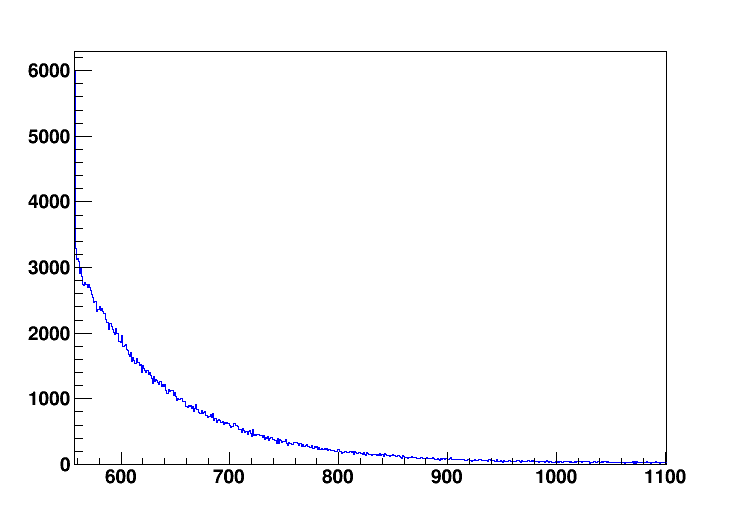
\includegraphics[width=\textwidth]{figures/FastOR/expoLongGap.png}};
%    \draw[red,ultra thick,rounded corners] (7.5,5.3) rectangle (9.4,6.2);
%    \draw[red, dashed,very thick, rotate=0] (2,1) --(2,3) -- (2,5);
%\end{tikzpicture}

%\begin{figure}[htbp!]
%\centering
%\begin{minipage}{.49\textwidth}
%  \centering
%	\includegraphics[width=1.0\textwidth]
%	{figures/FastOR/expoLongGap.png}
%	%\begin{tikzpicture}
%%    \node[anchor=south west,inner sep=0] at (0,0) {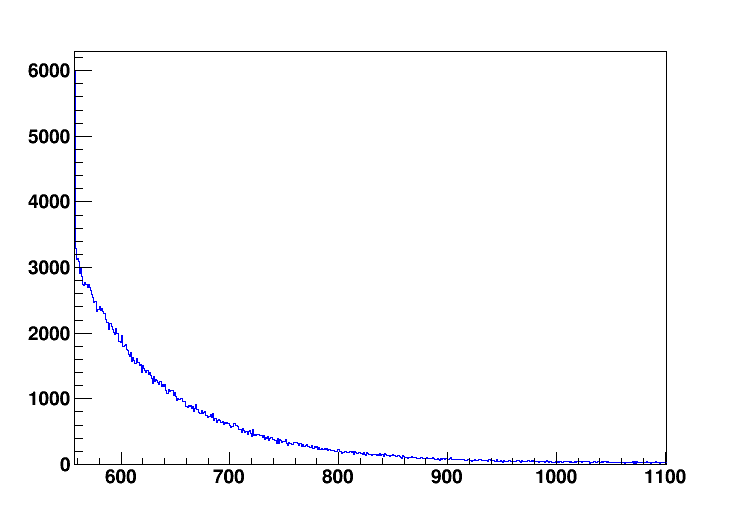
\includegraphics[width=\textwidth]{figures/FastOR/expoLongGap.png}};
%%    \draw[red, dashed,very thick, rotate=0] (1.01,0.5) --(1.01,3) -- (1.01,4);
%%    \draw [ ->] (5,3) -- (15,3);
%%	\end{tikzpicture}
%%    	    \caption{Coincidences vs BX}
%	    \label{fig:forLT}
%
%\end{minipage}%
%\begin{minipage}{.49\textwidth}
%  \centering
%	  \includegraphics[width=1.0\textwidth]%
%	    {figures/FastOR/expoShortGap.png}% picture filename
%%	    \caption{Coincidences vs BX, LCB}
%  \label{fig:forST}
%
%\end{minipage}
%    	    \caption{Contribution from non-colliding bunches}
%\end{figure}


\begin{figure}[htbp!]
  \includegraphics[width=1.0\textwidth]%
   {figures/FastOR/expoLongGap.png}
       \captionsetup{format=hang}    
    \caption{Exponential drop in contribution from non-colliding bunches as a function of bunch separation from the last filled bunch}
      \label{fig:forLT}

\end{figure}



Figure \ref{fig:forLT} shows the exponential decay in contribution as a function of separation between bunches. The first non-colliding bunch is at ~0.1\% of the preceding colliding bunch. Except for the first non-colliding BX immediately after filled BX, exponential drop (defined by tau of $\approx$ 90 BX) can be seen for all gaps. As such, contributions from non-colliding bunches is extremely low.





